\chapter{Una alimentación equilibrada}\label{ch:g3:balanced-diet}

Una obra necesita ladrillos, cemento, tablones --- y combustible para
las máquinas. Tu cuerpo es una obra que no cierra nunca: crece, se
repara y corre por ahí todo el día. Sus entregas llegan tres o cuatro
veces al día, en un plato. ¿Qué tienen que traer esas entregas? Esa es
la pregunta de la alimentación.

\section{Por qué el cuerpo necesita comida}

\begin{proposition}[Las dos tareas de la comida]\label{prop:g3:balanced-diet:jobs}
La comida hace dos tareas distintas:
\begin{enumerate}
  \item aporta \emph{energía}\index{energía (de los alimentos)} ---
        la fuerza para moverse, para mantenerse caliente, para que
        sigan funcionando el corazón y el cerebro, incluso durmiendo;
  \item aporta \emph{material de construcción} --- lo que el cuerpo
        usa para crecer en altura, para hacer \omterm{def:g3:bones-and-muscles:muscle}{músculo} y \omterm{def:g3:bones-and-muscles:skeleton}{hueso}, para
        curar rasguños y para reponer las piezas gastadas.
\end{enumerate}
Una alimentación tiene que entregar las dos cosas, todos los días.
\end{proposition}
\admitted

\begin{example}[Combustible incluso en reposo]\label{ex:g3:balanced-diet:rest}
Incluso tumbado sin moverte gastas \omterm{prop:g3:balanced-diet:jobs}{energía}: el corazón late, el pecho
sube y baja, el cuerpo se mantiene caliente a unos
$\qty{37}{\degreeCelsius}$ haga el tiempo que haga. Ese gasto fijo es
la razón de que saltarse comidas te deje débil y con frío, y no solo
con hambre.
\end{example}

\section{Las familias de alimentos}

\begin{definition}[Las familias de alimentos]\label{def:g3:balanced-diet:families}
Los alimentos se clasifican en \emph{familias de
alimentos}\index{familia de alimentos} según lo que aportan:
\begin{itemize}
  \item \emph{fruta y verdura} --- vitaminas, fibra y agua; la familia
        de la frescura;
  \item \emph{cereales y féculas} (pan, pasta, arroz, patatas) --- la
        familia de la \omterm{prop:g3:balanced-diet:jobs}{energía} que dura;
  \item \emph{lácteos} (\omterm{def:g2:animals-grow-up:born}{leche}, yogur, queso) --- la familia que
        construye los \omterm{def:g3:bones-and-muscles:skeleton}{huesos};
  \item \emph{carne, pescado y \omterm{def:g2:animals-grow-up:born}{huevos}} --- la familia que construye el
        cuerpo;
  \item \emph{grasas} (mantequilla, aceite) --- \omterm{prop:g3:balanced-diet:jobs}{energía} concentrada,
        necesaria en poca cantidad;
  \item \emph{alimentos dulces} --- un gusto rápido, nada necesario:
        la familia de los caprichos;
  \item y el \emph{agua}\index{agua (bebida)} --- la única bebida que
        el cuerpo necesita, durante todo el día.
\end{itemize}
\end{definition}

\begin{omfigure}
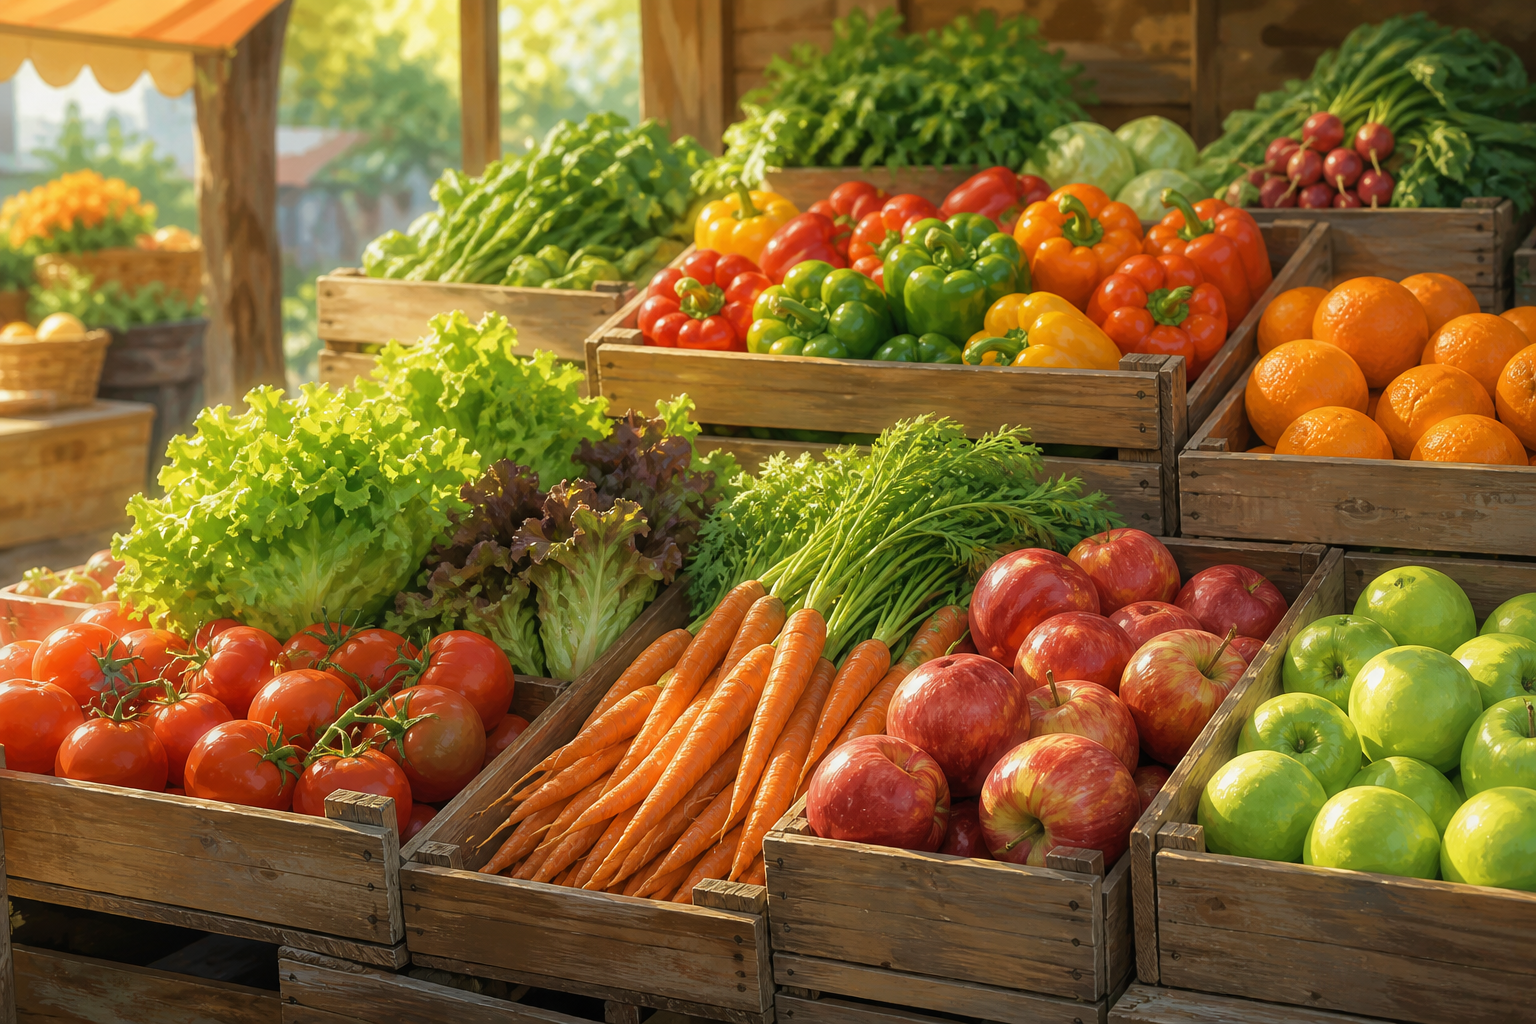
\includegraphics[width=0.62\linewidth]{images/book1/ai/g3-diet-market.png}

{\small La familia de la frescura en el mercado: el rincón del plato
que más se olvida, aquí sin ningún peligro de pasar desapercibido.}
\end{omfigure}

\begin{omfigure}
\begin{tikzpicture}
  % plate
  \draw[thick] (0,0) circle (2.8);
  % half: vegetables/fruit
  \draw[thick, fill=omMeth!14] (0,0) -- (0,2.8)
    arc[start angle=90, end angle=270, radius=2.8] -- cycle;
  % quarter: starchy
  \draw[thick, fill=omProp!14] (0,0) -- (0,-2.8)
    arc[start angle=270, end angle=340, radius=2.8] -- cycle;
  % quarter: builders
  \draw[thick, fill=omThm!12] (0,0) -- ({2.8*cos(340)},{2.8*sin(340)})
    arc[start angle=-20, end angle=90, radius=2.8] -- cycle;
  \node[font=\small, align=center] at (-1.4,0.2)
    {fruta y\\ verdura\\ (medio plato)};
  \node[font=\small, align=center] at (1.0,-1.45)
    {pan,\\ pasta, arroz};
  \node[font=\small, align=center] at (1.3,1.0)
    {carne, pescado,\\ huevo o lácteos};
  % water glass
  \draw[thick] (4.0,-0.5) -- (4.1,1.0) -- (5.0,1.0) -- (5.1,-0.5)
    -- cycle;
  \fill[omDef!25] (4.04,-0.44) -- (4.12,0.75) -- (4.98,0.75)
    -- (5.06,-0.44) -- cycle;
  \node[font=\small, align=center] at (4.55,-1.0) {agua};
\end{tikzpicture}

{\small Un plato bien equilibrado: media frescura, un cuarto de
\omterm{prop:g3:balanced-diet:jobs}{energía} que dura, un cuarto de constructores --- y agua en el vaso.}
\end{omfigure}

\begin{example}[Equilibrar una comida]\label{ex:g3:balanced-diet:lunch}
Pasta con salsa de tomate, un trozo de pescado, judías verdes, un
yogur, una manzana, agua: todas las familias presentes, los caprichos
ausentes --- una comida equilibrada. Patatas fritas, un refresco y una
chocolatina alimentan exactamente a dos familias (grasas y azúcar) y
se saltan las que la obra estaba esperando.
\end{example}

\begin{remark}[No hay alimentos prohibidos, solo olvidados]\label{rem:g3:balanced-diet:balance}
El equilibrio se mide en días, no en bocados sueltos. Un trozo de
tarta de cumpleaños no rompe ninguna regla --- el problema no es nunca
un capricho, sino los caprichos \emph{en lugar de} las familias, día
tras día. La pregunta práctica en cada comida no es ``¿es malo este
alimento?'' sino ``¿qué familia se me ha olvidado hoy?''.
\end{remark}

\section{Ajustar la comida al día}

\begin{proposition}[Las necesidades cambian con el día y con la persona]\label{prop:g3:balanced-diet:needs}
Cuánta \omterm{prop:g3:balanced-diet:jobs}{energía} necesita un cuerpo depende de quién es y de lo que
hace: un niño que crece necesita proporcionalmente más material de
construcción que una persona mayor; un día de deporte o de frío
invernal quema más \omterm{prop:g3:balanced-diet:jobs}{energía} que una tarde de lectura. El hambre crece
con el gasto del cuerpo.
\end{proposition}
\admitted

\begin{example}[Por qué importa el desayuno]\label{ex:g3:balanced-diet:breakfast}
Al llegar la mañana, el cuerpo lleva toda la noche funcionando ---
corazón, respiración, calor --- sin ninguna entrega. El desayuno lo
reabastece para las clases de la mañana y para las carreras. Sáltatelo
y a media mañana la obra se queda corta: tripas que suenan, atención
que se va, ninguna fuerza para jugar.
\end{example}

\begin{method}[Repasar el equilibrio de un día]\label{met:g3:balanced-diet:check}
Al final del día, repasa la lista:
\begin{enumerate}
  \item ¿fruta o verdura en cada comida? (objetivo: unas cinco
        raciones al día)
  \item ¿féculas en cada comida, para la \omterm{prop:g3:balanced-diet:jobs}{energía} que dura?
  \item ¿están los constructores --- lácteos varias veces y carne,
        pescado o \omterm{def:g2:animals-grow-up:born}{huevos} una o dos?
  \item ¿el agua como bebida del día?
  \item ¿los caprichos en poca cantidad y no como plato principal?
\end{enumerate}
Sea cual sea la familia que falte, invítala mañana.
\end{method}

\section{Ejercicios}

\begin{exercise}[$\star$]\label{exo:g3:balanced-diet:1}
¿Cuáles son las dos tareas de la comida? Da una \omterm{def:g3:balanced-diet:families}{familia de alimentos}
que sirva sobre todo a cada tarea.
\end{exercise}

\begin{exercise}[$\star$]\label{exo:g3:balanced-diet:2}
Nombra las \omterm{def:g3:balanced-diet:families}{familias de alimentos} y la única bebida que el cuerpo necesita.
\end{exercise}

\begin{exercise}[$\star$]\label{exo:g3:balanced-diet:3}
Clasifica esta compra en familias: arroz, yogur, zanahorias, \omterm{def:g2:animals-grow-up:born}{huevos},
mantequilla, manzanas, pan.
\end{exercise}

\begin{exercise}[$\star$]\label{exo:g3:balanced-diet:4}
¿Por qué gasta \omterm{prop:g3:balanced-diet:jobs}{energía} el cuerpo incluso mientras duerme? Nombra dos
de los gastos de la noche.
\end{exercise}

\begin{exercise}[$\star$]\label{exo:g3:balanced-diet:5}
Comprueba la comida ``pasta, pescado, judías verdes, yogur, manzana,
agua'' con el plato equilibrado de la figura: ¿qué parte del plato es
cada cosa?
\end{exercise}

\begin{exercise}[$\star$]\label{exo:g3:balanced-diet:6}
¿Por qué es especialmente importante el desayuno? ¿Qué pasa a media
mañana sin él?
\end{exercise}

\begin{exercise}[$\star$]\label{exo:g3:balanced-diet:7}
¿Quién necesita proporcionalmente más material de construcción: un
niño o una persona mayor? ¿Por qué?
\end{exercise}

\begin{exercise}[$\star$]\label{exo:g3:balanced-diet:8}
Pruébalo: pásale el \cref{met:g3:balanced-diet:check} a tu propio día,
con sinceridad. ¿Qué familia se te olvidó --- y cuál apareció más de
la cuenta?
\end{exercise}

\begin{exercise}[$\star\star$]\label{exo:g3:balanced-diet:9}
``¡Los dulces están prohibidos!'' ¿Es eso lo que dice este capítulo?
Da la regla más precisa de la \cref{rem:g3:balanced-diet:balance}.
\end{exercise}

\begin{exercise}[$\star\star$]\label{exo:g3:balanced-diet:10}
En unas vacaciones de esquí, todo el mundo tiene más hambre que en
casa. Explícalo con la \cref{prop:g3:balanced-diet:needs} --- nombra
los dos gastos añadidos que trae un día frío y deportivo.
\end{exercise}
